\chapter{Communication}\label{cha:communication}

As stated in the introduction, the force feedback loop should at least have a frequency of 550 Hz. This loop not only includes the communication between the Geomagic Touch and the computer but also the communication between the sbRIO and the computer and the computation time required for force estimation. In the current setup, the bottleneck is the communicating between the sbRIO and the computer as it can not exceed 100 Hz. As the drivers communication with the Geomagic Touch have a refresh rate of 1000 Hz and the computation time should be small compared to the refresh rate, the frequency of the communication with the embedded system should be at least 1200 Hz. However, from experimentation it was found out that the built-in library for UDP on the sbRIO cannot handle a frequency higher than 1000 Hz. If this maximum frequency is reached, the feedback loop will have a refresh rate of 500 Hz, see \figref{fig:speed_graph}, which is still deemed acceptable according to \cite{coles2011role}.  This chapter focuses on improving this communication to reach 1000 Hz.

\begin{figure}[H]
	\centering
	\begin{figure}
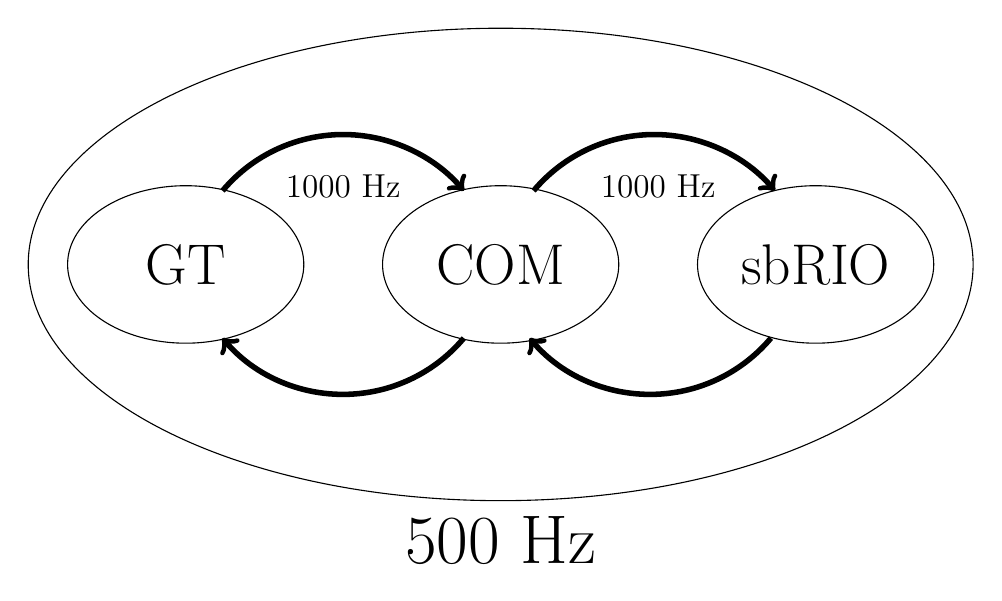
\begin{tikzpicture}

\draw  (-3,0) ellipse (1.5 and 1)node (v1) {\huge COM};
\draw  (-7,0) ellipse (1.5 and 1)node{\huge GT};
\draw  (1,0) ellipse (1.5 and 1)node{\huge sbRIO};


\draw [->,line width=2pt](-6.5321,0.9356) arc (139.9997:40:2);
\draw [<-,line width=2pt](-6.5321,-0.9356) arc (-139.9997:-40:2);
\draw [<-,line width=2pt](-2.6321,-0.9356) arc (-139.9997:-40:2);
\draw [->,line width=2pt](-2.5821,0.9356) arc (139.9997:40:2);


\node at (-5,1) {\large 1000 Hz};
\node at (-1,1) {\large 1000 Hz};
\draw  (v1) ellipse (6 and 3);
\node at (-3,-3.5) {\Huge 500 Hz};
\end{tikzpicture}

\end{figure}
	\caption{Communication loops inside the feedback loop}
	\label{fig:speed_graph}
\end{figure}

\section{TCP/IP}\label{sec:def_tcpip}

TCP/IP is a connection orientated protocol, which first establish the connection between two devices\cite{TCP_IP_UDP}. After the connection has been established data can be send in both directions. TCP/IP is a reliable protocol which ensure that the data transmitted, will be received. When the data is send, the transmitter waits for an acknowledgment from the receiver that the data has been received. If the data has been corrupted or the acknowledgment is not send, the transmitter will retransmit the package again. If the case of no acknowledgment is happening, a timer is used to define when to retransmit the data again. The data will then be retransmitted a certain amount of times until an acknowledgment has been received or the connection is defined to be disconnected. This means that a copy of the data is stored at the transmitter until it has been correctly received or the connection is taken down.\\
This communication protocol induces a delays in the system as the transmitter has to wait on the acknowledgment that the data has been received before loading new data into the sending buffer. If data has been discarded due to error the transmitter has to retransmit the data again if necessary.  


\section{ROS}\label{sec:ros}

In order to communicate between ROS and the sbRIO board the university created a ROS node called davinci\_driver. This driver is composed of three parts:
\todo{The university didn't create anything!}

\begin{itemize}
\item Low level driver
\item Middle level driver
\item High level driver
\end{itemize}
\todo{Itemizer need reference to Git repo}

The low level driver communicates directly with the sbRIO board. The high level driver handles the communication between ROS nodes. It updates the data for the nodes and transmits the setpoints to the low level driver through the middle driver. The name "setpoint" is used to designate the next position a motor should take.

The middle level driver handles both the creation of the low lever driver(s) and the communication between the low and high level driver so that there is no need for the client, ROS in our system, to acquire mutexes. Since it is possible to create more than one low level driver it is possible to communicate with more than one arm of the DaVinci robot.

The low level driver connects to one sbRIO board using a TCP/IP socket and exchange data with it using \gls{JSON} files, see \secref{subsec:JSON}. As shown in ~\figref{fig:original_driver}, the driver begins with an initialization of the connection and then start a loop. This loop is started in a thread and will run as long as the node is running. At each iteration of the loop, if some new data are present in the stream they are read and an update function is called to make them available to the higher levels. Then if there is some new setpoints or motor enable they are sent to the sbRIO. Finally, the thread goes to sleep before the next iteration of the loop. This sleeping period is introduced as to not overload the communication channel or the processor and this is the only control available on the speed of the communication.

\begin{figure}[H]
\centering
\begin{tikzpicture}

\node[box] (Initialization) at (0,0) {Initialization};
\node[box] (Receive) at ($(0,-2)+(Initialization)$) {Read the data \\if some were received};
\node[box] (Send) at ($(0,-2)+(Receive)$) {Send if the\\ control changed};
\node[box] (Sleep) at ($(0,-2)+(Send)$) {Sleep};
\node[box] (Update_State) at ($(5,0)+(Receive)$) {Update the data\\ available for higher\\level processes};

\draw[->, ultra thick] (Initialization) -- (Receive);
\draw[->, ultra thick] (Receive) -- (Update_State);
\draw[->, ultra thick] (Receive) -- (Send);
\draw[->, ultra thick] (Send) -- (Sleep);
\draw[->, ultra thick] (Sleep.west) -| ++(-2,0) |- (Receive);

\end{tikzpicture}
\caption{Structure of the original sbRIO driver}
\label{fig:original_driver}
\end{figure}


% The middle level driver allows the creation of more than one low level driver. Due to this it is possible to communicate with more than one arm of the DaVinci Robot at once. It also handles the communication between the high level driver and the low level so that there is no need for the client to acquire mutexes.\todo{last sentence - half of it is double confetti}

\subsection{sbRIO}\label{sec:sbrio}

%\todo{it would be nice to have a simple block diagram of the TCD, Data out/in and Debug/data loop. If we have the time do this!}

The sbRIO code running in the former setup has four code loops running in parallel. Since the sbRIO uses a single-core processor, the execution order depends on the operating system's decision, and can have stochastic characteristics. The four separated loops have distinct functions:

\begin{itemize}
	\item TCP connection loop for communicating with the ROS node
	\item Data out loop for reading data out of the FPGA
	\item Data in loop for setting FPGA parameters according to the received JSON packet
	\item Debug/data logging loop
\end{itemize}

The debug/data logging loop is not used during normal execution. The TCP loop communicates with the data loops through queues. It uses one queue for the received data, one for data out. The queues have only one element. When an enque attempt is made, the previous element is discarded and the newer one takes its place, ensuring that the queue always has the most up-to-date element.

The TCP communication is set up serially, i.e. the sbRIO sends data then waits for incoming data. It is a timed loop, thus the code attempts to run once in each specified period. When the loop is executing for the first time or when it experiences error, it creates/recreates a TCP connection using a TCP listener. After that, the loop reads the data out queue, if it finds an element in it, it sends it through the TCP connection. Then it polls for incoming data. When it arrives, the loop enques the data in the received data queue. Then it restarts the process.

When the user stops the execution, the connection is terminated.

\chapter{Improvement}\label{cha:improvement}
\todo{Rewrite introduction}

%\section{Minimum refresh speed}\label{sec:min_speed}

The refresh rate for the force feedback has an influence on the transparency of the controller. An ideal situation is that there is no delay in the system and the system is perfectly modeled, thus give the user a direct feedback of the forces the tool is exposed to.\\ 
The force can also be scaled if high precision task is to be made, thus increase the resistance the operator is fed from the feedback.
\todo{maybe scaled? and Update rate vs. delay. Also jitter should be considered} 

{\color{green}
As one of the goals for this project is to implement a force feedback controller, the requirement for the force feedback speed should be met. Thus the bandwidth of the communication speed should be increased.
} 

{\color{red} 
As one of the goals for this project is to increase the bandwidth for the communication and thereby enable the opportunity of making a force feedback control, the required refresh rate of a 1000 Hz should be met.
}
% From the article \textit{The role of haptics in medical training simulators: a survey of the state of the art}\cite{coles2011role}, it is said that the minimum refresh rate of haptic feedback is wildly debated to be between 300 Hz and 600 Hz, but for a realistic force feedback it is commonly accepted to be at least 1000 Hz, thus it is not defined. \todo{This is just marked with a "!" sign by Christoffer}

From \secref{sec:prev_communication} the communication between the sbRIO and the computer was in the previous setup running at 100 Hz, which does not meet the requirement of a 1000 Hz. Therefore the speed should be raised with at least a factor of ten. It is however preferable to exceed this so the system does not run on the limit, thus having the ability to make complex calculations.


\subsection*{Approach}
Speeding up the communication could be done in different ways, where three are stated below

\begin{itemize}
	\item Find a faster communication protocol,
	\item Minimize the amount of data transmitted,
	\item Implement faster hardware.	
\end{itemize}

Implementing faster hardware is not a possibility in this case as one of the goals for this project is to only use the existing hardware.
\todo{This is not written anywhere?}
However implementing a new communication protocol and minimizing the package size is possible.\\
\todo{What will we test in the following sections..small tail to this introduction would be nice for the flow }
% Implementing faster hardware does however not match with the goals of this project as one of them being to use only the existing hardware.\todo{This is not written anywhere?} 


% As stated in \secref{sec:com_ROS_sbRIO}, the current communication is set to run at a frequency of 100 Hz and to do a force feedback we need more than 300 Hz, see \secref{sec:min_speed}. This means that it is required to find a way to speed up the communication in order to do a force feedback. Speeding up the communication could be done by three different ways:

% \begin{itemize}
% 	\item Find a faster communication protocol,
% 	\item Minimize the amount of data transmitted,
% 	\item Implement faster hardware.	
% \end{itemize}
% \todo{More analyses is required}

% Implementing faster hardware does not match with the goals of our project one of them being to use only the existing hardware.\todo{This is not written anywhere?}
% However, finding a communication protocol faster than TCP/IP is possible as the safeties in the protocol tend to slow down the overall speed of the communication\todo{we need a ref for this}. Furthermore, some of the safeties like congestion control are irrelevant in our case since we are directly connected to the destination. Flow control is not necessary as the need for flow control implies that a delay is created on the receiving side which would induce delay in the entire system. Reliable transport and ordered delivery are a problem, since retransmitting data is useless in our case as the data will be deprecated. Instead, it is much more interesting to receive the new data. 

% The protocol chosen for this project is \gls{UDP}. This is done because its a faster protocol than TCPI/IP and the project goal is to reduce the latency in communication between the computer running ROS and the sbRIO board. It is however less relaible than TCP/IP but it is deemed irrelevant as a new package with data should be send send as soon as possible. This also solve the problem with storing old data in the transmitter buffer which could be obsolete.
\section{Protocol}\label{sec:Protocol}

Finding a communication protocol faster than TCP/IP is possible as the safeties in the protocol tend to slow down the overall speed of the communication\todo{we need a ref for this}. Furthermore, some of the safeties like congestion control are irrelevant in our case since we are directly connected to the destination. Flow control is not necessary as the need for flow control implies that a delay is created on the receiving side which would induce delay in the entire system. Reliable transport and ordered delivery are a problem, since retransmitting data is useless in our case as the data can be deprecated. Instead, it is much more interesting to receive new data. 

The protocol chosen for this project is \gls{UDP}. This is done because its a faster protocol than TCPI/IP and the project goal is to reduce the latency in communication between the computer running ROS and the sbRIO board. It is however less reliable than TCP/IP but it is deemed irrelevant to some extent as a new package with data should be send as soon as possible. This also solve the problem with storing old data in the transmitter buffer which could be obsolete. Even though it is deem irrelevant that \gls{UDP} is a less reliable protocol and package lose can appear, it is still necessary to include safety in the system if an connection error should appear.  


% As stated in \secref{sec:com_ROS_sbRIO}, the current communication runs at a frequency of a 100 Hz and to do a force feedback, a minimum of 300 Hz is needed, see the introduction to \chapref{cha:improvement}. This means that it is required to find a way to speed up the communication in order to do force feedback. Speeding up the communication could be done in different ways, where three is stated below

% \begin{itemize}
% 	\item Find a faster communication protocol,
% 	\item Minimize the amount of data transmitted,
% 	\item Implement faster hardware.	
% \end{itemize}

% As stated in \secref{sec:com_ROS_sbRIO}, the current communication is set to run at a frequency of 100 Hz and to do a force feedback we need more than 300 Hz, see \secref{sec:min_speed}. This means that it is required to find a way to speed up the communication in order to do a force feedback. Speeding up the communication could be done by three different ways:

% \begin{itemize}
% 	\item Find a faster communication protocol,
% 	\item Minimize the amount of data transmitted,
% 	\item Implement faster hardware.	
% \end{itemize}


% Implementing faster hardware does not match with the goals of our project one of them being to use only the existing hardware.\todo{This is not written anywhere?}




\subsection{Minimizing the size of the transmitted messages}\label{subsec:minimizing}
% \todor{I proposed a new text for this part, it is in color}
% To minimize the forwarded data size, first of all we have to get rid of the names of each data. To keep the data readable for the receiver, we can either use a character to separate each segment of data, or we can agree upon a constant size for each segment of data.

% The former code encoded each digit of a decimal number as an ASCII character. It means that the number segment only used 10 out of the 256 possible characters. To compress data, we should utilize all the ASCII characters. One way to do it is to make a character store the number as its address in the 8 bit address table. We basically have to convert the numbers to base 256.

% We utilized Labview's \todo{maybe we should move it to implementation} built in flatten to string node, which basically converts numeric data to the correspondent string. For example, it convert an 8 bit integer to the correspondent ASCII character. If the sbRIO and the PC uses the same encoding, they can basically send bitcode as if it was string then decode it by doing a simple conversion.
 
% \todo{please specify formally the new and old protocol}

% For each arm, the sbRIO must send encoder, potmeter and current measurement data from each of the seven motors. Each data is represented as a 32 bit float. This adds up to 48 bytes of data to be sent each cycle. The described method sends 48 byte long strings not including the header. The former method sends 67 characters for formatting and naming purposes and 96 bytes of numeric data, assuming each double number is sent in 8 digits. It adds up to 163 bytes.

% By removing the names from the string and compressing a data, the string can become 70 percents shorter, which is a valuable increase in efficiency.

%%%%%%%%%%%%%%%%%%%%%%%%%%%%%%%%%%%%%%%%%%%%%%%%%%%%%%%%%%%%

There are two elements that impact greatly the size of the exchanged messages: the number of character added by the JSON format and the length of the numbers.
As detailed in ~\secref{subsec:JSON}, the JSON format add numerous characters for the structure and require a name for each value. The first modification made in order to minimize the size of the messages was to remove the JSON format. One way of doing this is to define a fixed format for the messages. For simplicity, it was decided to keep a format similar to the original one, composed of a vectors of positions, velocities and efforts. All of these vectors contain the same number of elements and each elements must have the same length to make it possible to read. 
With the original \gls{JSON} format it is possible to specify the content of the file using the name of the first element in it. In addition to the messages containing the positions, velocities and efforts, there is messages that can be sent to indicate which motors are active or not. In order to implement that feature in the new format a byte is added at the end of the packet, this byte contains a boolean for each motors indicating if the motor is active or not.

As mentioned, all the numbers in the vectors should have the same length. In the original format, not only the numbers were long (18 digits) but the length would vary from one message to another. Different solutions were considered. The first one would be to fix the number of digits but that would still imply a conversion to string. The second solution considered was the compression of the characters sent. 

 However the compression rate generally is not higher than 50\% for random data and the computation time induced by compression would results in an additional delay instead of decreasing the existing one \cite{simple_compression}\cite{fast_ZIV}. The third and last option was to send the binary representation directly without any encoding. The numerical values being stored as floats, each of them requires 4 bytes. It have the advantage of having a fixed length without having to round the value. The last solution was chosen as it has the lowest computation time, since no encoding is used. The only issue is that the endianness of both devices is not the same, this is corrected in the implementation on the ROS side. The packets obtained with the new format are shown in \figref{fig:new_packets}.%The packets obtained with the new format are shown in \tabref{fig:received_packet} and \tabref{fig:sent_packet}

With the original format, the packet described in \secref{subsec:JSON} contained 346 characters. With the new format, the packet that contains the same information is 49 bytes. Therefore, the packets following the new format uses 15\% of the original size.
\begin{figure}[h]
\centering
\begin{tikzpicture}
    \matrix(dict)[matrix of nodes,%below=of game,
        nodes={align=center,text width=1.5cm},
        row 1/.style={anchor=south}%,
        column 1/.style={nodes={text width = 0.5cm, align=right}}
    ]{
		0 	& position1 & position2 & position3 & position4\\
		16 	& velocity1 & velocity2 & velocity3 & velocity4\\
		32 	& effort1 	& effort2 	& effort3 	& effort4\\
		48	\\
    };
    %horizontal
    \draw(dict-1-2.north west)--(dict-1-5.north east);
    \draw(dict-1-2.south west)--(dict-1-5.south east);
    \draw(dict-2-2.south west)--(dict-2-5.south east);
    \draw(dict-3-2.south west)--(dict-3-5.south east);
	%vertical
    \draw(dict-1-1.north east)--(dict-4-1.south east);
    \draw(dict-1-2.north east)--(dict-3-2.south east);
    \draw(dict-1-3.north east)--(dict-3-3.south east);
    \draw(dict-1-4.north east)--(dict-3-4.south east);
    \draw(dict-1-5.north east)--(dict-3-5.south east);

    %small at bottom
    \draw(dict-4-1.south east)--($(0.5,0)+(dict-4-1.south east)$);
    \draw($(0.5,0)+(dict-4-1.south east)$)--($(0.5,0.49)+(dict-4-1.south east)$);

    %numbers on top
    \node at ($(0,0.3)+(dict-1-1.north east)$) {0};
    \node at ($(0,0.3)+(dict-1-2.north east)$) {4};
    \node at ($(0,0.3)+(dict-1-3.north east)$) {8};
    \node at ($(0,0.3)+(dict-1-4.north east)$) {12};
    \node at ($(0,0.3)+(dict-1-5.north east)$) {16};

    \node at ($(0,0.3)+(dict-1-1.north)$) {bytes};
    \node at ($(0,0.6)+(dict-1-1.north)$) {Offset};

    %The zoom on the last byte
    \node (zoom) at (1,-2) {XXXX 4 booleans};
    \draw(zoom.north east)--(zoom.north west);
    \draw(zoom.north east)--(zoom.south east);
    \draw(zoom.north west)--(zoom.south west);
    \draw(zoom.south east)--(zoom.south west);
    \draw($(zoom.north)+(-0.25,0)$)--($(zoom.south)+(-0.25,0)$);
    \draw(zoom.north east)--($(1,0)+(dict-4-1)$);
    \draw(zoom.north west)--($(1,0)+(dict-4-1)$);
    \node at ($(zoom.north east)+(0,0.3)$) {1};
    \node at ($(zoom.north west)+(0,0.3)$) {0};

\end{tikzpicture}
\caption{Packet , built using the binary representation}
\label{fig:new_packets}
\end{figure}
% With the original format, one message such as the one in ~\secref{subsec:JSON} contained 583 characters (583 bytes) for 7 motors. With the new format the message that contains the same information is 85 bytes. Therefore, the messages following the new format uses only 15\% of the original size.

%%%%%%%%%%%%%%%%%%%%%%%%%%%%%%%%%%%%%%%%%%%%%%%%%%%%%%%%%%%%
% \begin{table}[H]
% \centering
% \begin{tabular}{| l | l | l | l | l |}
%   \hline			
%   				 & Positions & Velocities & Efforts & Active\\ \hline
% Number of floats & 7 		 & 7 		  & 7 		& 		\\ \hline
% Number of bytes  & 4$\cdot$7 		 & 4$\cdot$7 		  & 4$\cdot$7 	& 1		\\
% \hline  
% %\caption{Packet from the sbRIO to ROS for one arm, with a payload size of 85 bytes.}
% %\label{fig:received_packet}
% \end{tabular}
% \caption{Packet from the sbRIO to ROS for one arm, with a payload size of 85 bytes.}
% \label{fig:received_packet}
% \end{table}
% %\todo{What is the resolution of the encoders compared to the representation
% 	%\\ the sbrio can provide 2048 ticks per rotation. it comes down to around 18000 ticks between the two endpoints of the motor}

% \begin{table}[H]
% \centering
% \begin{tabular}{| l | l | l |}
% \hline			
% 					& Set points	 & Enabled\\ \hline
% Number of floats	& 7				 &		  \\ \hline
% Number of bytes		& 7$\cdot$4 bytes		 & 1 byte \\
% \hline  
% %\caption{Packet from ROS to the sbRIO for one arm, with a payload size of 29 bytes.}
% %\label{fig:sent_packet}
% \end{tabular}
% \caption{Packet from ROS to the sbRIO for one arm, with a payload size of 29 bytes.}
% \label{fig:sent_packet}
% \end{table}


% \begin{figure}[H]
% \centering
%  \resizebox {\linewidth} {!} {
% \begin{tikzpicture}

% \draw (0,0) rectangle (17,1);
% \draw (0,0) rectangle (5,1);
% \draw (0,0) rectangle (10,1);
% \draw (0,0) rectangle (15,1);

% \node at (2.5,0.5) {Positions};
% \node at (7.5,0.5) {Velocities};
% \node at (12.5,0.5) {Efforts};
% \node at (16,0.5) {Active};

% \node at (2.5,-0.5) {\textbf{7 floats}};
% \node at (7.5,-0.5) {\textbf{7 floats}};
% \node at (12.5,-0.5) {\textbf{7 floats}};
% %\node at (16,-0.5) {\textbf{n booleans}};

% \node at (2.5,-1) {7*4 bytes};
% \node at (7.5,-1) {7*4 bytes};
% \node at (12.5,-1) {7*4 bytes};
% \node at (16,-1) {1 byte};

% %\node at (4,-2.5) {\textbf{Size of the payload:} 85 bytes}; %I have no idea why i need to put 4 as a coordinate for it to not mess up the rest of the figure
% \end{tikzpicture}}
% \caption{Packet from the sbRIO to ROS for one arm, with a payload size of 85 bytes.}
% \label{fig:received_packet}
% \end{figure}




% \begin{figure}[H]
% \centering
% \resizebox {\linewidth} {!} {
% \begin{tikzpicture}

% \draw (0,0) rectangle (10,1);
% \draw (0,0) rectangle (7,1);

% \node at (3.75,0.5) {Setpoints};
% \node at (8.5,0.5) {Enabled};

% \node at (3.75,-0.5) {\textbf{7 floats}};
% %\node at (8.5,-0.5) {\textbf{n booleans}};

% \node at (3.75,-1) {7*4 bytes};
% \node at (8.5,-1) {1 byte};

% %\node at (0,-2.5) {\textbf{Size of the payload:} 29 bytes}; 
% \end{tikzpicture}}
% \caption{Packet from ROS to the sbRIO for one arm, with a payload size of 29 bytes.}
% \label{fig:sent_packet}
% \end{figure}

\section{Implementation}
The improvements described in \secref{cha:improvement} need to be implemented on both ROS's and sbRIO's side \todo{somthing needed here!!}


\subsection{ROS side}

In order to implement in ROS the improvements described to increase the speed of the communication it is necessary to write a new driver. As previously explained, the new driver should use \gls{UDP} instead of TCP/IP. It should also transmit the actual data without using a \gls{JSON} Stream so that the size of each packets is reduced. In addition to those objectives it would be better to modify as little as possible the current structure of the ROS node so that it does not have to be fully rewritten. 
Three goals that need to be fulfilled when writing the new driver were defined. The goals are stated below:
\begin{enumerate}
	\item Replace TCP by UDP
	\item Replace the \gls{JSON} Stream by the numerical values
	\item Modify as little as possible the original driver
\end{enumerate}

The modifications that need to be made in order to carry duty 1. and 2. are related to the communication protocol and the format of the transmitted data which are both handled by the low level driver. In order to fulfill goal 3. only the low level driver should be modified without having consequences on the higher level drivers. This means that the public functions should keep the same prototype and that the format of the data available for them should stay the same (i.e vectors of double). The boost library should be used as it was in the original driver, to handle threads and mutexes.

The socket initialization for the \gls{UDP} protocol is very close to the one made for TCP protocol, thanks to this the establishment of the communication with the sbRIO is similar in both the old and new drivers. However, the \gls{UDP} being connectionless it is not possible to use the same method as before to read incoming data, i.e it is not possible to look if some new data arrived, with \gls{UDP} it is necessary to constantly be listening for new incoming data. In a first time, a new code structure was implemented. This new structure ran two threads, one for receiving data and one for sending. However when the frequency of the communication increased towards 1000Hz the packets were sent by two and received by two instead of sending one and receiving one. In order to cancel this it was decided to use a single thread as in the original driver. 

To use a single thread it is necessary to modify the receive function as the default one for UDP is blocking, i.e. it waits until it receives a packet before the code can continue. Thus, a new funtion was defined, that function blocks only for a specified amount of time to received a packet, if nothing is received the loop can continue. With this new function it is possible to use a single thread and thus to keep full control over the order in which the packets are sent and received.

As shown in ~\figref{fig:new_driver}, the new driver starts with an initialization of the connection and of the data structure and then starts a loop. As in the original driver this loop will run as long as the driver is running. In each iteration, if there is some new setpoints or motor enables, a message is sent to the sbRIO. Then, the new receive function is called, if a message is received the bitcode is converted to the actual values and made available to the higher levels, if no message is received before the deadline, the code continues. Finally, the thread goes to sleep as the original one did. Once again this sleep controls the frequency of the communication, however, in this new driver the waiting time of the receive function and the \gls{RTT} delay also impact the frequency. 
%  That is why the communication loop is to be modified so that it is always waiting to receive a packet and that it sends data when required. However, if the communication loop shown in \figref{original_driver} was used, the loop would be blocking if no packet was received. To solve this issue a new thread is created that will wait to receive a packet, handle the packet and start again. This new communication structure is shown in \figref{new_driver}.

 As explained before, when the \gls{JSON} Stream was removed it was decided that only send numerical data would be sent. And as goal 3. is kept in mind, it is needed to receive the position, velocity and effort as float and one boolean for each motor and to send a setpoint as a double and a boolean for each motor. The received values must be made available as double for the higher levels by storing them in the vector of doubles. For simplicity it was decided that the packet should be following the structure described in \figref{fig:new_packets}. To reach the desired vectors, the received bitcode stored in an array of char is copied in a float variable that is converted in a double and then the value in the vector is updated using this double. As the endianness of the sbRIO is not the same as the one used on most computer, when the bitcode is copied to the float variable the order of the bytes is reversed (the first byte becomes the last one).

The structure of the sent packet is shown in~\figref{fig:sent_packet}. To build the packet, the same logic as before is used. The bitcode of the numerical values is copied into an array and the array is sent.
In regards to the boolean values, they are stored in a byte with 1 bit per value which is possible only because the number of motors for one arm is 7 (i.e inferior to 8 which is the maximum amount of booleans that could be stored in 1 byte).

\begin{figure}[H]
\centering
\begin{tikzpicture}

\node[box] (Initialization) at (0,0) {Initialization};
\node[box] (Check_Send) at ($(0,-2.5)+(Initialization)$) {Check if there is\\new data to send};
\node[box] (Send) at ($(0,-2.5)+(Check_Send)$) {Send};
\node[box] (Receive) at ($(0,-2.5)+(Send)$) {Timed receive};
\node[box] (Check_Receive) at ($(0,-2.5)+(Receive)$) {Check if a packet\\was received};
\node[box] (Handle) at ($(0,-2.5)+(Check_Receive)$) {Convert the bitcode\\and make data available\\to higher levels};
\node[box] (Sleep) at ($(0,-2.5)+(Handle)$) {Sleep};


\draw[->, ultra thick] (Initialization) -- (Check_Send);
\draw[->, ultra thick] (Check_Send) -- (Send);
\draw[->, ultra thick] (Send) -- (Receive);
\draw[->, ultra thick] (Receive) -- (Check_Receive);
\draw[->, ultra thick] (Check_Receive) -- (Handle);
\draw[->, ultra thick] (Handle) -- (Sleep);

\draw[->, ultra thick] (Check_Send.east) -- ++(1,0) |- (Receive.east);
\draw[->, ultra thick] (Check_Receive.east) -- ++(1,0) |- (Sleep.east);
\draw[->, ultra thick] (Sleep.west) -| ++(-2,0) |- (Check_Send);



\node at ($(2.1,0.2)+(Check_Send)$) {No};
\node at ($(0.4,-1)+(Check_Send)$) {Yes};

\node at ($(2.1,0.2)+(Check_Receive)$) {No};
\node at ($(0.4,-1)+(Check_Receive)$) {Yes};

\end{tikzpicture}
\caption{Structure of the new low level driver}
\label{fig:new_driver}
\end{figure}


% \begin{figure}[H]
% \centering
% \begin{tikzpicture}

% \node[box] (Initialization) at (4,0) {Initialization};
% \node[box] (Receive) at ($(4,-3)+(Initialization)$) {Wait to receive\\a packet};
% \node[box] (Update_State1) at ($(0,-3)+(Receive)$) {Convert the bitcode};
% \node[box] (Update_State2) at ($(0,-3)+(Update_State1)$) {Make the data available for\\higher level processes};

% \node[box] (Check) at ($(-4,-3)+(Initialization)$) {Check if there is\\a new control signal};
% \node[box] (Send) at ($(0,-3)+(Check)$) {Send};
% \node[box] (Sleep) at ($(0,-3)+(Send)$) {Sleep};


% \draw[->, ultra thick] (Initialization.south) -- ++(0,-0.5) -|  (Receive.north);
% \draw[->, ultra thick] (Receive) -- (Update_State1);
% \draw[->, ultra thick] (Update_State1) -- (Update_State2);
% \draw[->, ultra thick] (Update_State2.west) -| ++(-1,0) |- (Receive);

% \draw[->, ultra thick] (Initialization.south) -- ++(0,-0.5) -| (Check);
% \draw[->, ultra thick] (Check) -- (Send);
% \draw[->, ultra thick] (Check.east) -| ++(0.5,0) |- (Sleep);%($(0,1.5)+(Sleep)$);
% \draw[->, ultra thick] (Send) -- (Sleep);
% \draw[->, ultra thick] (Sleep.west) -| ++(-1.5,0) |- (Check);

% \node at ($(0,2.1)+(Check)$) {\textbf{thread1}};
% \node at ($(0,2.1)+(Receive)$) {\textbf{thread2}};

% \node at ($(2.1,0.2)+(Check)$) {No};
% \node at ($(0.4,-1)+(Check)$) {Yes};

% \end{tikzpicture}
% \caption{Structure of the new sbRIO driver}
% \label{new_driver}
% \end{figure}
% \todo{We still need to define the initialization protocol and the packet loss handling}

The driver described is functional, however there is one feature of the TCP/IP that was useful to our system and that we lost by switching to UDP: the connection timeout detection. As safety is essential in this system, it is necessary to implement an additional layer to the communication to make it more reliable. To implement this safety we have two options: using a free library or implement our own safety protocol. The free libraries that can be found include UDT\cite{UDT} and ENet\cite{ENet}. Those libraries provide a reliable option for long distances communication by adding a number of features. However on the ROS side, it is only necessary to alarm the user of the connection timeout. For such a simple purpose, the free libraries would add to many features that are superfluous in this system and thus slow down the communication. That is why we chose to implement our own safety protocol.

 In order to do so, we decided to add a counter to the current driver. Every time the receive function reaches its deadline, the counter is incremented. Every time a packet is received, the counter is reseted. When the receive function reaches its deadline, in addition to the incrementation, the value of the counter is tested. If the value is superior to 10 (this value is arbitrary), en error is thrown and displayed to the user to notify of the connection timeout. The new code structure is shown in ~\figref{fig:new_safe_driver}




\begin{figure}[H]
\centering
\begin{tikzpicture}

\node[box] (Initialization) at (0,0) {Initialization};
\node[box] (Check_Send) at ($(0,-2.5)+(Initialization)$) {Check if there is\\new data to send};
\node[box] (Send) at ($(0,-2.5)+(Check_Send)$) {Send};
\node[box] (Receive) at ($(0,-2.5)+(Send)$) {Timed receive};
\node[box] (Check_Receive) at ($(0,-2.5)+(Receive)$) {Check if a packet\\was received};
\node[box] (Reset) at ($(0,-2.5)+(Check_Receive)$) {Reset the counter};
\node[box] (Handle) at ($(0,-2.5)+(Reset)$) {Convert the bitcode\\and make data available\\to higher levels};

\node[box] (Sleep) at ($(0,-2.5)+(Handle)$) {Sleep};

\node[box] (Increment) at ($(4.5,0)+(Reset)$) {Increment the counter};
\node[box] (Timeout) at ($(4.5,0)+(Handle)$) {if counter > 10,\\throw error};


\draw[->, ultra thick] (Initialization) -- (Check_Send);
\draw[->, ultra thick] (Check_Send) -- (Send);
\draw[->, ultra thick] (Send) -- (Receive);
\draw[->, ultra thick] (Receive) -- (Check_Receive);
\draw[->, ultra thick] (Check_Receive) -- (Reset);
\draw[->, ultra thick] (Reset) -- (Handle);
\draw[->, ultra thick] (Handle) -- (Sleep);

\draw[->, ultra thick] (Check_Send.east) -- ++(0.75,0) |- (Receive.east);
\draw[->, ultra thick] (Check_Receive.east) -| (Increment.north);
\draw[->, ultra thick] (Increment) -- (Timeout);
\draw[->, ultra thick] (Timeout.south) |- (Sleep);

\draw[->, ultra thick] (Sleep.west) -| ++(-2,0) |- (Check_Send);



\node at ($(2.1,0.2)+(Check_Send)$) {No};
\node at ($(0.4,-1)+(Check_Send)$) {Yes};

\node at ($(2.1,0.2)+(Check_Receive)$) {No};
\node at ($(0.4,-1)+(Check_Receive)$) {Yes};

\end{tikzpicture}
\caption{Structure of the new low level driver with connection timeout detection}
\label{fig:new_safe_driver}
\end{figure}
 %In order to do so, we decided to add a counter to the current driver. Every time the thread1 check if some data should be sent, the counter is increased by one. Every time a packet is received, the counter is reset to 0 in thread2. In addition to incrementing the counter the thread1 will test the value, if it is superior to 10 (arbitrary value), a message is sent to indicate the packet loss. If the value is superior to 20, a message is sent to indicate connection timeout and the system on ROS is shut down. The new code structure is shown in ~\figref{new_safe_driver}

% \begin{figure}[H]
% \centering
% \begin{tikzpicture}

% \node[box] (Initialization) at (4,0) {Initialization};
% \node[box] (Receive) at ($(4,-3)+(Initialization)$) {Wait to receive\\a packet};
% \node[box] (Reset_Counter) at ($(0,-3)+(Receive)$) {Reset the counter};
% \node[box] (Update_State1) at ($(0,-3)+(Reset_Counter)$) {Convert the bitcode};
% \node[box] (Update_State2) at ($(0,-3)+(Update_State1)$) {Make the data available for\\higher level processes};

% \node[box] (Check) at ($(-4,-3)+(Initialization)$) {Check if there is\\a new control signal};
% \node[box] (Send) at ($(0,-2.5)+(Check)$) {Send};
% \node[box] (Increment) at ($(0,-2.5)+(Send)$) {Increment the counter};
% \node[box] (Connection_Timeout) at ($(0,-2.5)+(Increment)$) {if counter > 10\\throw an error};
% \node[box] (Sleep) at ($(0,-2.5)+(Connection_Timeout)$) {Sleep};


% \draw[->, ultra thick] (Initialization.south) -- ++(0,-0.5) -|  (Receive.north);
% \draw[->, ultra thick] (Receive) -- (Reset_Counter);
% \draw[->, ultra thick] (Reset_Counter) -- (Update_State1);
% \draw[->, ultra thick] (Update_State1) -- (Update_State2);
% \draw[->, ultra thick] (Update_State2.west) -| ++(-1,0) |- (Receive);

% \draw[->, ultra thick] (Initialization.south) -- ++(0,-0.5) -| (Check);
% \draw[->, ultra thick] (Check) -- (Send);
% \draw[->, ultra thick] (Check.east) -| ++(0.75,0) |- (Increment);%($(0,1.5)+(Sleep)$);
% \draw[->, ultra thick] (Send) -- (Increment);
% \draw[->, ultra thick] (Increment) -- (Connection_Timeout);
% \draw[->, ultra thick] (Connection_Timeout) -- (Sleep);
% \draw[->, ultra thick] (Sleep.west) -| ++(-1.5,0) |- (Check);

% \node at ($(0,2.1)+(Check)$) {\textbf{thread1}};
% \node at ($(0,2.1)+(Receive)$) {\textbf{thread2}};

% \node at ($(2.1,0.2)+(Check)$) {No};
% \node at ($(0.4,-1)+(Check)$) {Yes};

% \end{tikzpicture}
% \caption{Structure of the new sbRIO driver with connection timeout detection}
% \label{new_safe_driver}
% \end{figure}


\subsection{Embedded System}
\label{Embedded}
\subsubsection{sbRIO Microprocessor}

The processor on the sbRIO board is running at a 400 MHz clockrate, while our target communication frequency is 1 kHz. This means that the code running on the processor has to be optimized in order to achieve the set goals. The fundamental functions of the sbRIO are the following:

\begin{itemize}
	\setlength\itemsep{0em}
	\item Read data from the FPGA, converting position values based on the gearing
	\item Encode the data into a string
	\item Send the string through a UDP port
	\item Fix communication errors
	\item Poll incoming UDP packets, send the decoded values to the FPGA
	\item Emergency shutdown	
\end{itemize}


The code includes tools for debugging and measurement, these have a substantial impact on the communication performance. They are disabled during normal operation. LabView's array handling is far from optimal, further speed increase could be achieved by compiling a more optimized C code into a DLL file and calling it in the LabView code. The extra functionalities are the following:

\begin{itemize}	
	\setlength\itemsep{0em}
	\item Timestamp sender through UDP
	\item Time logging for packet departure and arrival to csv file
	\item Front Panel PID gain adjustment, motor enabler
	\item Manual, sinusoidal, squarewave signal generator for the motor
	\item Motor data logging to csv file
	
\end{itemize}

We need to decide how to handle connection loss. Either we turn of the motors or we stay in position.

\subsubsection{FPGA}

The FPGA built into the sbRIO is taking care of the interfacing between the controllers and the microprocessor. The code running on the FPGA is much faster than the one running on the microprocessor. To reach maximum possible speed, we implemented whatever we could on the FPGA, however the FPGA is incapable of handling higher level functions such as string handling and UDP networking.

The FPGA's main functions are the following:

\begin{itemize}	
	\setlength\itemsep{0em}
	\item Count the encoder ticks coming from the controller
	\item Read the controller's analog and digital inputs 
	\item Calculate position PID control signal and send the corresponding PWM signal to the controller
	\item Enable the motors
	
\end{itemize}

Since the current value coming from the ESCON is noisy, the FPGA also needs a built in low pass filter.

\subsubsection{ESCON motor controllers}

The ESCON controllers are programmed to output a speed corresponding to the FPGA PWM signal. The speed controller has an inner current controller, which also keeps the motors from taking overcurrent. The current ramps can be adjusted to fit the user's needs. The speed control gain can be adjusted by the onboard potmeter. 
The outer speed loop provides the control signal for the internal current controller. The inner control loop must have a higher frequency than the speed control loop. The PI current controller is running at 53.6 kHz, while the PI speed controller is running at 5.36 kHz. The inner loop ensures fast response, the outer higher precision ($http://www.iraj.in/journal/journal_file/journal_pdf/1-59-140229369778-81.pdf$). The advantages of the cascade structure:

\begin{itemize}
	\item Better setpoint tracking
	\item Better disturbance rejection
	\item Less delay and phase lag
\end{itemize}

The position is controlled by setting the duty ratio of the incoming PWM signal. The speed reference is 0 at 50\% duty ratio and grows linearily at higher values.
The ESCON controller has 2 programmable analog outputs, thus we are unable to read speed, actual current and demand current simultaneously.
The controllers have autocalibration functionalities, but this ability is obstructed by the gearing limits.


Look into whether we can read data from the ESCON controllers!



\section{Software architecture}
\todor{Filip is this correct?}

\gls{ROS} is an open source software development tool for implementing robotics software. It provides the opportunity of hardware abstraction, low level device control, implementation of commonly used functionalities, messages between different processes and package management\cite{wiki_ros}. It provide tools and libraries which utilize the the opportunity of communicating between disturbed computers, obtaining, writing and running codes.

\todoc{When we make a reference to e.g Wiki\_ROS, there is no author available. Is it okay to just write the Author as "Robotic operating systems" or how do we do this?}

\GLS{ROS} has three different levels of concepts\cite{Wiki_ros_concepts}

\begin{itemize}
\item Filesystem level
\item Computation graph level
\item and the Community level
\end{itemize}

\subsection*{File system level}
The file system level takes care of package management between different nodes 
\subsection*{Computation graph level}

\subsection*{Community level}


% ROS is an open-source, meta-operating system that handles
% hardware abstraction, low-level device control, implementation
% of commonly-used functionality, message-passing between
% processes, and package management.

%  It also provides tools and libraries for obtaining, building, writing, and running code supporting distributed computing. At the file system level, the main organizational component of a ROS system
% is the package. A package may contain executables (nodes),
% libraries, data-sets and configuration files. In a robot control
% system, nodes process data and communicate with each other
% through the Computation Graph.\todo{Still NO references...}

% The Computation Graph is the peer-to-peer network of ROS
% processes that are processing data together. Communication
% is done by nodes subscribing to and publishing standardized
% data structures called messages by way of topics. Topics can
% be seen as a location for a certain type of message to be
% subscribed and published to. Possibly the greatest advantage
% ROS has on other similar projects is the community. Most of
% the packages are community maintained by a large and active
% user base, which makes the process of learning the system
% considerably easier.

\section*{Structure}

In a high level overview, our system could structurally be represented in several components.
The sBRio board controls the actuators on the DaVinci robot arm and the rest of the system communicates with it via drivers contained in the Davinci\_ ros package. The Phantom Omni communicates with the system via the Open Haptics API, and connects to ROS through the phantom\_ omni package.

Connecting all the system components requires an architecture based on a central node which handles communication between the two packages and has access to all the other methods required for control.
We have developed the Endohap package exactly for this purpose.
The endohap\_ node node contained in the package connects all the main system components using protocols either defined by ROS (TCP/IP) or externally (UDP). 

Communication with the Endowrist test setup is handled by the boost libraries in the davinci\_ drivers package. 
The sbrio\_ driver program transforms the data received by UDP and propagates it through the system using internal ROS communication protocols and vice versa. 
More precisely, the motor state data is poblished to the joint\_ states ROS topic, which the central (endohap) node is subscribed to.
Since this makes it is possible to use a separate (non-ROS) protocol for communicating with the test setup while maintaining ROS protocols for the internal system, we conclude that this approach gives a higher degree of control in terms of communication speed.

The motor state data is then used by the endohap node for Endowrist external force estimation and feedback generation.
After this is done, the resulting force feedback reference needs to be sent to the phantom\_ omni package, from which the endohap node also recieves the user input for the Endowrist. While the phantom\_ omni package handles hardware communication via external TCP/IP protocols, the endohap node only publishes and subscribes to appropriate topics in order to communicate with that part of the system.

All the calculation required for controlling the endowrist and giving force feedback to the phantom omni is also done within the endohap node. Forward kinematics are handled by the tf ROS package, which utilizes URDF description files combined with current joint position information published to ROS.
This consequently allows for other useful features such as visualization in Rviz or various kinematics calculations.
Forming the node in an object-oriented manner gives the added advantage of modularity, allowing for implementation of additional features as they become necessary. 

\begin{figure}[H]
\centering
\begin{tikzpicture}
%Peripheral
\draw (0,2) rectangle (7.6,10);
\node [box] (ECOM) at (3.8,8.5) {Endowrist COM};
\node [box] (EEST) at ($(0,-2) + (ECOM)$) {Endowrist \\ state estimation};
\node [box] (ECTRL) at ($(-2,-3) + (EEST)$) {Endowrist \\ control};
\node [box] (REFBK) at ($(2,-3) + (EEST)$) {Reference \\ and feedback};
\node [box] (OMNI) at ($(4,0) + (REFBK)$) {phantom\_ omni};
\node [box] (PHANTOM) at ($(0,-2) + (OMNI)$) {Phantom \\ Omni};
\node [box] (DAVINCI) at ($(6,0) + (ECOM)$) {davinci\_ driver};
\node [box] (TEST) at ($(0,-2) + (DAVINCI)$) {Test setup};

\draw[->, ultra thick] (ECOM) -- (EEST);
\draw[<-, ultra thick] (EEST) -- ($(0,-1.2) + (EEST)$);
\draw[-, ultra thick] ($(0,-1.2) + (EEST)$) -- ($(-2,-1.2) + (EEST)$);
\draw[->, ultra thick] ($(-2,-1.2) + (EEST)$) -- (ECTRL);
\draw[-, ultra thick] ($(0,-1.2) + (EEST)$) -- ($(2,-1.2) + (EEST)$);
\draw[->, ultra thick] ($(2,-1.2) + (EEST)$) -- (REFBK);
\draw[->, ultra thick] (REFBK) -- (ECTRL);
\draw[<->, ultra thick] (REFBK) -- (OMNI);
\draw[<->, ultra thick] (OMNI) -- (PHANTOM);
\draw[<->, ultra thick] (ECOM) -- (DAVINCI);
\draw[<->, ultra thick] (DAVINCI) -- (TEST);
%\draw[->, ultra thick] (helper) -- (REFBK);


\end{tikzpicture}%
\caption{simple Tikz figure}
\end{figure}


\section{Measurements}

\section{TCP measurements}\label{sec_tcp_mes}

\subsection*{Purpose:}

To determine the maximum frequency that can be used with the TCP/IP protocol. To do so, we will measure the round time trip delay and jitter and look at those values as a function of the delay used in the sending loop.

\subsection*{Test equipment:}

The sbRIO 9636 is connected to a computer running Ubuntu 14.04 LTS via an Ethernet cable of 1 gpbs\todo{check the speed}. The computer runs the ROS nodes that are used for the project, thus it communicates with both the Geomagic Touch and the sbRIO and it sends random setpoints to the sbRIO. The sbRIO uses the entire code of the project.

\subsection*{Procedure:}

\begin{enumerate}
	\item The sbRIO is started and connected to the computer.
	\item The ROS node is started and ran for at least 60 seconds. 
	\item The log files are retrieved to be analyzed using Matlab.
\end{enumerate}
Those steps are repeated for the following settings: 10 ms, 2 ms and 0 ms.


\subsection*{Measuring data:}

The times at which a packet was received or sent are recorded in files through the sbRIO driver on the computer.

\subsection*{Results:}

\begin{center}
	$\begin{tabular}{c|ccccc}
		Delay & \text{Sending frequency} & \text{Receiving frequency} & \text{Average delay} & Jitter & \text{Error rate}\\
		\hline
		10ms & 4 & 4 & 1 & 1 & 1 \\
		2ms & 4 & 4 & 1 & 1 & 1 \\
		0ms & 4 & 4 & 1 & 1 & 1 \\
	\end{tabular}$
	\captionof{table}{TCP}
\end{center}


\subsection*{Uncertainties of measurement:}

??

\subsection*{Conclusion:}

Hopefully UDP is faster.

\section{UDP measurements}\label{sec_udp_mes}

\subsection*{Purpose:}

To determine the maximum frequency that can be used with the UDP protocol. To do so, we will measure the round time trip delay and jitter and look at those values as a function of the delay used in the sending loop. For the UDP protocol we take measurements for two configurations: one with the sending and receiving serialized on the sbRIO and one with both done in parallel using separate threads. 

\subsection*{Test equipment:}

The sbRIO 9636 is connected to a computer running Ubuntu 14.04 LTS via an Ethernet cable of 1 gpbs\todo{check the speed}. The computer runs the ROS nodes that are used for the project, thus it communicates with both the Geomagic Touch and the sbRIO and it sends random setpoints to the sbRIO. The sbRIO uses the entire code of the project.

\subsection*{Procedure:}

\begin{enumerate}
	\item The sbRIO is started and connected to the computer.
	\item The ROS node is started and ran for at least 60 seconds. 
	\item The log files are retrieved to be analyzed using Matlab.
\end{enumerate}
Those steps are repeated for both the serial and parallel case for the following settings: 10 ms, 5 ms, 3 ms, 2.5 ms, 2 ms, 1.5 ms and 1 ms.


\subsection*{Measuring data:}

The times at which a packet was received or sent are recorded in files through the sbRIO driver on the computer.

\subsection*{Results:}
\begin{center}
	$\begin{tabular}{c|ccccc}
		Delay & \text{Sending frequency} & \text{Receiving frequency} & \text{Average delay} & Jitter & \text{Error rate}\\
		\hline
		10ms & 4 & 4 & 1 & 1 & 1 \\
		5ms & 2 & 1 & 4 & 1 & 1 \\
		3ms & 4 & 4 & 1 & 1 & 1 \\
		2.5ms & 4 & 4 & 1 & 1 & 1 \\
		2ms & 4 & 4 & 1 & 1 & 1 \\
		1.5ms & 4 & 4 & 1 & 1 & 1 \\
		1ms & 4 & 4 & 1 & 1 & 1 \\
	\end{tabular}$
	\captionof{table}{Serialized UDP}
\end{center}

\begin{center}
	$\begin{tabular}{c|ccccc}
		Delay & \text{Sending frequency} & \text{Receiving frequency} & \text{Average delay} & Jitter & \text{Error rate}\\
		\hline
		10ms & 4 & 4 & 1 & 1 & 1 \\
		5ms & 2 & 1 & 4 & 1 & 1 \\
		3ms & 4 & 4 & 1 & 1 & 1 \\
		2.5ms & 4 & 4 & 1 & 1 & 1 \\
		2ms & 4 & 4 & 1 & 1 & 1 \\
		1.5ms & 4 & 4 & 1 & 1 & 1 \\
		1ms & 4 & 4 & 1 & 1 & 1 \\
	\end{tabular}$
	\captionof{table}{Parallel UDP}
\end{center}

\subsection*{Uncertainties of measurement:}

??

\subsection*{Conclusion:}

Hopefully UDP is faster.